\documentclass[a4paper]{article}
\usepackage[UTF8]{ctex}
\usepackage{geometry}
\usepackage{graphicx}
\usepackage{url}
\usepackage{multirow}
\usepackage{array}
\usepackage{booktabs}
\usepackage{url}
\usepackage{enumitem}
\usepackage{graphicx}
\usepackage{float}
\usepackage{amssymb}
\usepackage{amsmath}
\usepackage{subfig}
\usepackage{longtable}
\usepackage{pifont}
\usepackage{color}

\allowdisplaybreaks

\geometry{a4paper, scale=0.78}

% \begin{figure}[H]
%     \centering
%     \includegraphics[width=.55\textwidth]{E.png}
%     \caption{矩阵与列向量的乘法}
%     
% \end{figure}

% \left\{
% \begin{array}{ll}
%       x+2x+z=2 & \\
%       3x+8y+z=12 & \\
%       4y+z=2
% \end{array}
% \right.

% \begin{enumerate}[itemindent = 1em, itemsep = 0.4pt, parsep=0.5pt, topsep = 0.5pt]

% \end{enumerate}

%\stackrel{a}{\longrightarrow}

%\underbrace{}_{} %下括号

\title{Gaussian Mixture Model 01 Model Introduction}
\author{Chen Gong}
\date{23 December 2019}

\begin{document}
\maketitle
这一章开始,我们将进入到Guassian Mixture Model (GMM)的学习。而为什么要学习GMM呢?这是因为单峰分布已经不能准备的反映数据的分布了。正如下面的一个分布:
\begin{figure}[H]
    \centering
    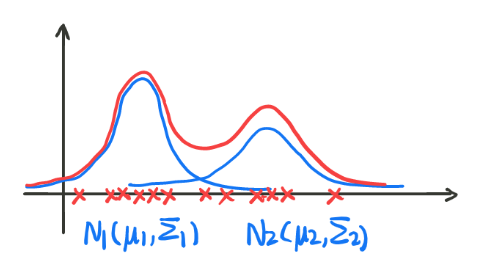
\includegraphics[width=.55\textwidth]{微信图片_20191223221952.png}
    \caption{数据分布举例}
    
\end{figure}

对于如上的数据分布来说,如果强行用单峰的Guassian Distribution来表示这个分布,显然是可以的。但是,很明显是不合适的。会造成较大的误差,不能较好的表示整个数据的分布特征。

\section{从几何角度来看}
从几何角度来看比较的简单,也就是多个高斯分布来取加权平均值。也就是一个混合高斯分布就是多个高斯分布叠加而成的。那么,概率密度函数,可以被我们写成:
\begin{equation}
    p(x) = \sum_{k=1}^K \alpha_k \mathcal{N}(\mu_k, \Sigma_k), \qquad \sum_{k=1}^K \alpha_k = 1
\end{equation}

\section{从混合模型角度来看(生成模型)}
如果当输入变量的维度高于一维的时候,我们就不能使用简单的加权来看了。因为,这时,我们已经无法简单的用加权平均来计算了,正如下图所示。其中,$X$是Observable Variable,$Z$是Latent Variable。这个$Z$是个什么意思呢?我们先举一个小例子。看到图2中那个打了红圈圈的数据点。它既属于$C_1$的分布,并且也属于$C_2$的分布,我们可以写作:
\begin{figure}[H]
    \centering
    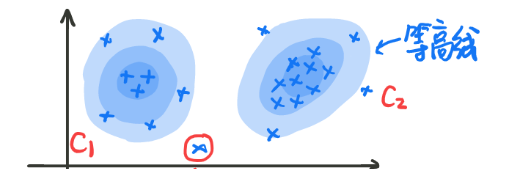
\includegraphics[width=.65\textwidth]{微信图片_20191223223203.png}
    \caption{二维数据分布举例}
    
\end{figure}

\begin{equation}
    \left\{
        \begin{array}{ll}
            X \sim C_1 & \\
            X \sim C_2  
        \end{array}
    \right.
\end{equation}

这样写太麻烦了,我们可以直接写成$X \sim Z$,这里的$Z$就是一个离散的随机变量,它包含了$C_1,C_2,\cdots,C_N$的概率分布,$Z$服从的是类别分布,其实就是看对应的样本$X$是属于哪一个高斯分布的概率。可以被我们写成:
\begin{table}[H]
    \centering
    \begin{tabular}{c|cccc}
         $Z$ & $C_1$ & $C_2$ & $\cdots$ & $C_k$  \\
         \hline
         $P(Z)$ & $P_1$ & $P_2$ & $\cdots$ & $P_k$  \\
    \end{tabular}
    \caption{隐变量$Z$的离散概率分布}
\end{table}

并且,$\sum_k P_k = 1$。接下来,我们来说一说,如何来生成$N$个样本点,$x_1,x_2,\cdots,x_N$。

我们假设有一个骰子,有$K$个面,每个面都是不均匀的,假设我们可以控制每一个面的质量,那么这个骰子的面出现的概率会符合某个分布。有$K$个面,就有$K$个高斯分布。那么每次我们就投一下这个骰子,根据出现的面$K$,选择在第$K$个高斯分布中进行采样,生成一个样本点$x_i$。

概率图可以被我们描述为如下形式:
\begin{figure}[H]
    \centering
    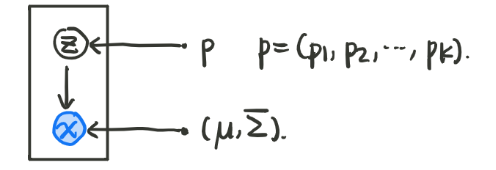
\includegraphics[width=.45\textwidth]{微信图片_20191223234640.png}
    \caption{GMM的概率图表达形式}
    
\end{figure}

我们根据一个离散的随机变量$Z$来选择是选取那个高斯分布,利用这个高斯分布$\mathcal{N}(\mu,\Sigma)$来采样得到我们想要的样本点。而且,离散随机变量$Z$符合一个离散分布$p = (p_1,p_2,\cdots,p_k)$。

\end{document}
